\section{Analysis}

In the following, we present an analysis of our notation, the models and the
taxonomy we generated.

\subsection{Notations}

I justified the notation we designed earlier as a simple, compact notation.
What I did not count upon was the bloated notation and whitespace required to
effectively denote processes.
This was especially evident in the V-Model (see Figure \ref{VModel}), where many
tiny tasks that were decomposed caused the diagram to expand to huge levels.
This made the model appear less simple, and went against the expected criteria
and use-cases I had expected when designing my notation.\\
\\
Of note is that every symbol that had been designed was used in some model.
This meant that the notation was suitably expressive in most cases, in that
every symbol had some useful meaning in some process.\\
\\
An informal suggestion from conversations with Terry Woodings resulted in his
suggestion that colour and aesthetics were a powerful part of effective
notations.
Unfortunately, there was not any time to explore this avenue, but I would like
to acknowledge it as one possible way to improve my notation as it stands.
It would be much easier on the eyes and possibly convey extra meaning in the
diagram.\\
\\
Finally, we note that perhaps the use of natural language ended up being a great
weakness of the notation. It made the models extremely large and they expanded
to unwieldy level and difficult to interpret sizes.\\
\\
I reproduce Figure \ref{VModel} for an interested reader to illustrate some of
the points I have made about my notation.

\begin{figure}
\centering
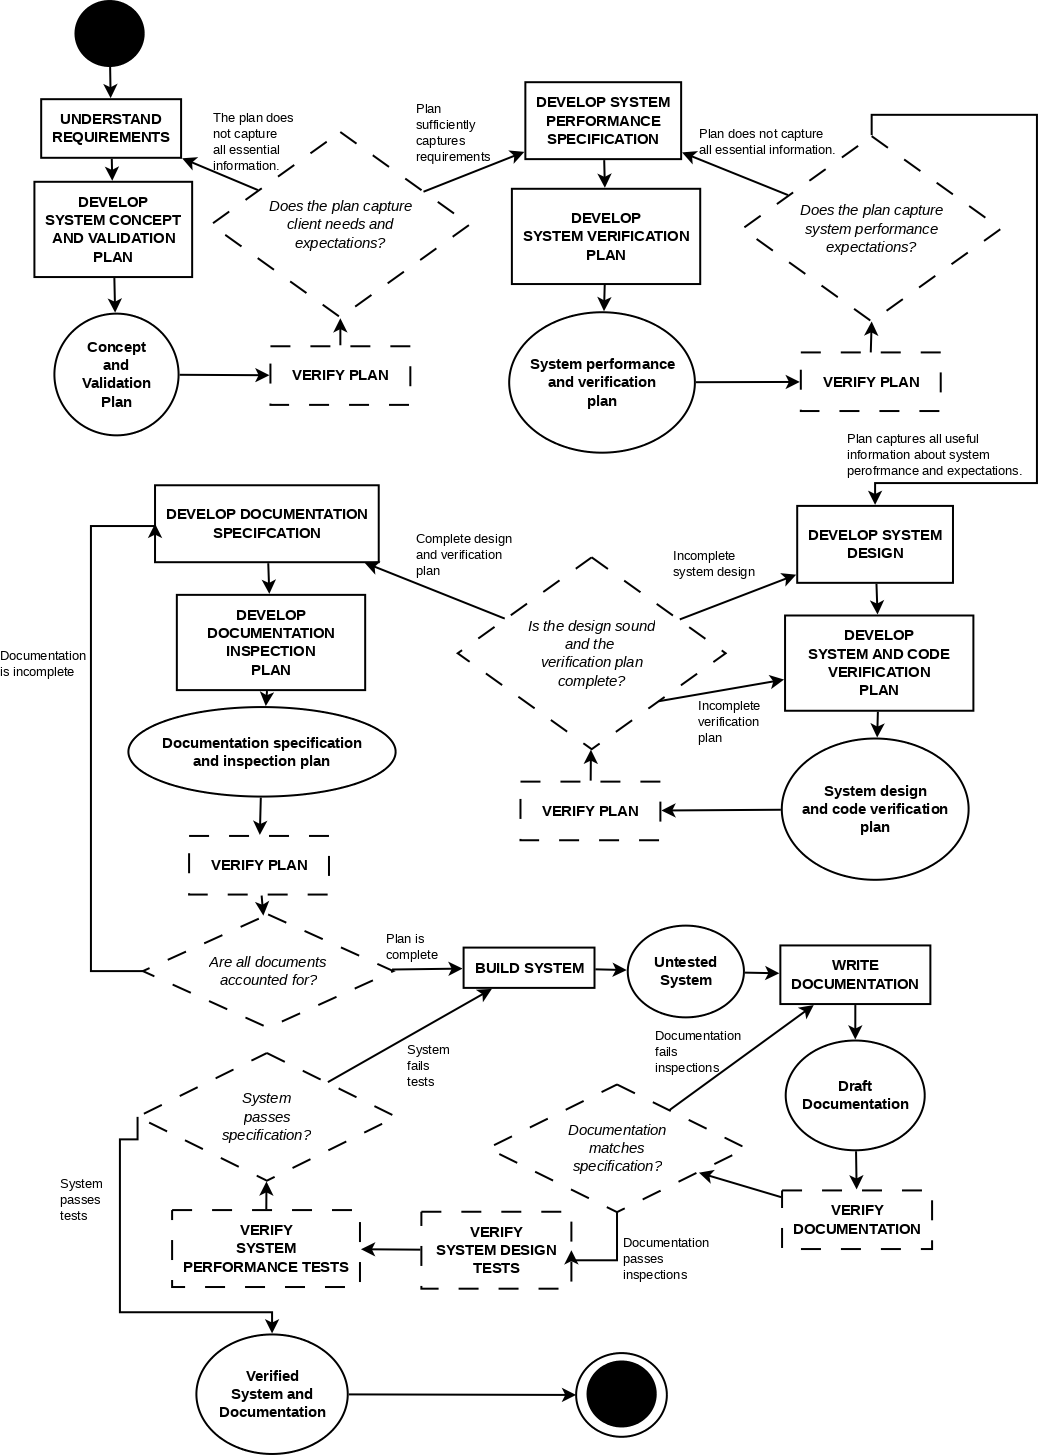
\includegraphics[scale=0.3]{media/VModel}
\caption{Three things about the notation that caused the model to be more
complex than needed were the 
verbosity of natural language,
lack of colour and aesthics as well as the 
 whitespace and large amounts of symbols used.}
\label{VModelAgain}
\end{figure}

\pagebreak

\subsection{Taxonomy}
We have already noted some weaknesses about our taxonomy.
It classified my single-developer process (Figure \ref{MyProcess}) to be the same as a multi-developer
process --- Crystal Clear (Figure \ref{CrystalClean}).
Although the adaption of a team process to a single deveoper process is
possible, it remains an open question of {\em why} this occurred.\\
\\
I believe it is a question of detail.
The notation I used was built around activities and capturing how processes and
activities occurred.
It was basic, due to its finding its roots in flowcharts and UML activity
diagrams \cite{Dumas01umlactivity, BellUMLBasics}.
Unfortunately, it fails to capture certain intricacies, such as culture changes,
resource changes and other semantic differences in meaning.\\
\\
The other criticism I could make is related to the choices of questions used in
my hierarchical partionings.
It was difficult to differentiate models in certain cases, and perhaps the
characteristics I chose were not effective in determining which models were
which.\\
\\
I noted the three interesting characteristics of classifying the models.\\
\\
Firstly, my belief is that all of the sequential models were the same.
Although I classified each one separately, I would consider it perhaps as good
or to say ``they are the same model".
They simply have tiny differences, such as a risk analysis stage or the demand
that a specific plan is written before implementation.
It is seemingly easy to turn the Waterfall model into the Spiral model ---
after each verification stage, perform a risk analysis to determine what
setbacks the project could suffer, and the models start to look very similar.
In reality, they appeared to all be the Waterfall model, except repackaged in an
attempt to overcome its shortcomings.
This seems sensible, since they are all from the same era of programming, when a
phase-based or Waterfall approach was the norm in all engineering disciplines.

\pagebreak

\begin{figure}[ht!]
  \centering
  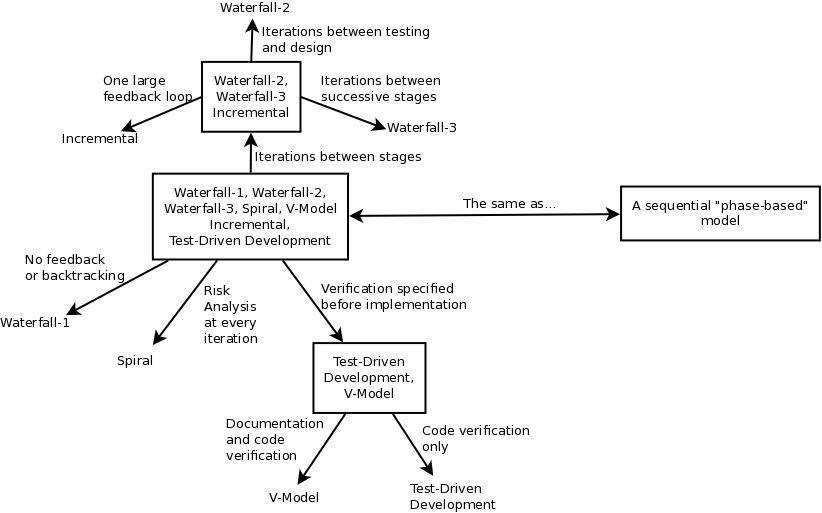
\includegraphics[scale=0.35]{media/DecisionTreeAllEqual}
  \caption{This is Figure \ref{DecTree4}, but here I make a comment that I
  would almost have considered the end point as ``a phase-based model".}
  \label{DecTreeAll}
\end{figure}

Secondly, as I noted earlier, I claimed that Scrum and Evolutionary
methodologies were similar enough to be in an equivalence class, and similarly
for Crystal Clear and Extreme Programming.
These equivalences were similar to my reasoning for why the sequential
``phase-based models" were similar.
What they represented to me was something much more interesting, which I discuss
in my third and final point.\\
\\
The last thing I noticed was two different philosophies within the agile
movement.
One still had elements of planning in it; it was a proactive, flexible planning
philosophy that both Crystal Clear and Extreme Programming practiced.
The other was an organic, feature driven philosophy that prioritised user needs
over planning and documentation.
Both had user interaction inbuilt into their methodology but it was interesting
to notice that these philosophical and documentation differences existed.

\begin{figure}[ht!]
  \centering
  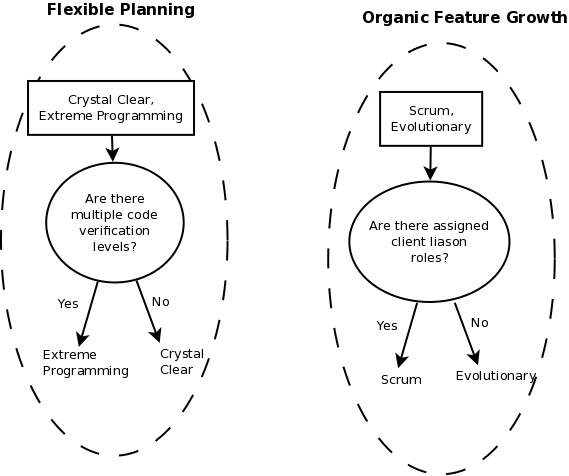
\includegraphics[scale=0.4]{media/DecisionTreeAgilers}
  \caption{The differing philosophies of evolution versus planned agile projects.
  Here, I give a rudimentary diagrammatic classification of four of the
  processes into either of the two philosophies.}
  \label{DecTreeAgilers}
\end{figure}

\pagebreak

\subsection{Automated Analyses}
One avenue that greatly interested me was the possibility of an automated
classifier for software processes.
I did not have sufficient time or resources to investigate it properly, but I
outline the problem as an open research question that could help later in
industry to determine useful methods or formal standards appropriate for a
project.\\
\\
Given a software process we would want to automatically classify what existing
methodology it most resembles.
This question involves
\begin{enumerate}
  \item translating the process into a formal notation
  \item performing an analysis on the process' structure and semantics
  \item classifying the process or scoring it based on its resemblance to an existing software
  development methodology
\end{enumerate}

Possible approaches I propose, without reference and simply as ideas, are
\begin{itemize}
  \item a decision tree learner, which would make a more advanced version of
  the classification scheme I constructed. An interesting question is to
  determine what are the ``good" discriminating characteristics, and if so why
  they are ideal for discrimination.
  \item Likert scale classification which suggests a numerical score of
  similarity (that is, construction of a similarity index).
  What these numbers actually mean is another matter!
  Whether this index could be useful is another matter entirely and I only
  propose it as an interesting possibility for this problem.
  \item graph based analysis for ``isomorphism" or ``similarity" based on
  structure of the process. This does not take into account the ``meanings"
  of the process, and is simply whether or not the structure of the process is
  similar.
  A counter-example for a naive graph isomorphism check would be similarities
  between the Spiral and Waterfall-3 models.
  However, there might be methods to overcome these with probabilistic or
  partial graph equivalence analyses.
  I again propose this as another open approach which is interesting, but one
  that is outside the scope of this paper.
\end{itemize}

\subsection{Further work}

In summary, from my analyses, I would highlight four possible avenues of future
work
\begin{enumerate}
  \item methodologies for ``prettier" or aesthetically pleasing notations using
  colour to convey meaning in a less verbose way
  \item an exploration of appropriate characteristics to use in decision trees
  during classification
  \item an exploration of structural analyses of models based on graph theory
  and model checking
  \item whether there are philosophical branches of agile that ascribe to
  either a planning or reactive methodology of software development
\end{enumerate}
